
% ----------------------------------------------------------------------
% Set the document class
% ----------------------------------------------------------------------
\documentclass[12pt	]{article}
\usepackage{multirow}
\usepackage{matlab-prettifier}



% ----------------------------------------------------------------------
% Define external packages, language, margins, fonts, new commands 
% and colors
% ----------------------------------------------------------------------
\usepackage[utf8]{inputenc} % Codification
\usepackage[english]{babel} % Writing idiom

\usepackage[export]{adjustbox} % Align images
\usepackage{amsmath} % Extra commands for math mode
\usepackage{amssymb} % Mathematical symbols
\usepackage{anysize} % Personalize margins
    \marginsize{2cm}{2cm}{2cm}{2cm} % {left}{right}{above}{below}
\usepackage{appendix} % Appendices
\usepackage{cancel} % Expression cancellation
\usepackage{caption} % Captions

    \DeclareCaptionFont{newfont}{\fontfamily{cmss}\selectfont}
    \captionsetup{labelfont={bf, newfont}}
\usepackage{cite} % Citations, like [1 - 3]
\usepackage{color} % Text coloring
\usepackage{fancyhdr} % Head note and footnote
    \pagestyle{fancy}
    \fancyhf{}
    \fancyhead[L]{\footnotesize \fontfamily{cmss}\selectfont Embedded Systems} % Left of Head note
    \fancyhead[R]{\footnotesize \fontfamily{cmss}\selectfont CE5439} % Right of Head note
    \fancyfoot[L]{\footnotesize \fontfamily{cmss}\selectfont CE Dep.} % Left of Footnote
    \fancyfoot[C]{\thepage} % Center of Footnote
    \fancyfoot[R]{\footnotesize \fontfamily{cmss}\selectfont AUT} % Right of Footnote
    \renewcommand{\footrulewidth}{0.4pt} % Footnote rule
\usepackage{float} % Utilization of [H] in figures
\usepackage{graphicx} % Figures in LaTeX
\usepackage[colorlinks = true, plainpages = true, linkcolor = blue, urlcolor = blue, citecolor = blue, anchorcolor = blue]{hyperref}
\usepackage{indentfirst} % First paragraph
\usepackage[super]{nth} % Superscripts
\usepackage{siunitx} % SI units
\usepackage{subcaption} % Subfigures
\usepackage{titlesec} % Font
    \titleformat{\section}{\fontfamily{cmss}\selectfont\Large\bfseries}{\thesection}{1em}{}
    \titleformat{\subsection}{\fontfamily{cmss}\selectfont\large\bfseries}{\thesubsection}{1em}{}
    \titleformat{\subsubsection}{\fontfamily{cmss}\selectfont\normalsize\bfseries}{\thesubsubsection}{1em}{}
    \fancyfoot[C]{\fontfamily{cmss}\selectfont\thepage}

% Random text (not needed)
\usepackage{lipsum}
\usepackage{duckuments}

% New and re-newcommands
\newcommand{\sen}{\operatorname{\sen}} % Sine function definition
\newcommand{\HRule}{\rule{\linewidth}{0.5mm}} % Specific rule definition
\renewcommand{\appendixpagename}{\LARGE \fontfamily{cmss}\selectfont Appendices}

% Colors
\definecolor{istblue}{RGB}{3, 171, 230}
\definecolor{dkgreen}{rgb}{0,0.6,0}
\definecolor{gray}{rgb}{0.5,0.5,0.5}

% Image path
\graphicspath{ {./Images/} }

\usepackage[most]{tcolorbox}

%%%%%%%%%%%%%%%%%%%%%%%%%%%%%%%%%%%%%%%%%% Solution box setting %%%%%%%%%%%%%%%%%%%%%%%%%%%%%%%%%%%%%%%%%%
\newtcbtheorem{Problem}{\bfseries Problem}{enhanced,drop shadow={black!50!white},
	coltitle=black,
	top=0.3in,
	attach boxed title to top left=
	{xshift=1.5em,yshift=-\tcboxedtitleheight/2},
	boxed title style={size=small,colback=pink}
}{summary}

\newtcolorbox[auto counter]{summary}[1][]{title={\bfseries Problem~\thetcbcounter},enhanced,drop shadow={black!50!white},
	coltitle=black,
	top=0.3in,
	attach boxed title to top left=
	{xshift=1.5em,yshift=-\tcboxedtitleheight/2},
	boxed title style={size=small,colback=pink},#1}
	
%%%%%%%%%%%%%%%%%%%%%%%%%%%%%%%%%%%%%%%%%%%%%%%%%%%%%%%%%%%%%%%%%%%%%%%%
%                                 Document                             %
%%%%%%%%%%%%%%%%%%%%%%%%%%%%%%%%%%%%%%%%%%%%%%%%%%%%%%%%%%%%%%%%%%%%%%%%
\begin{document}

% ----------------------------------------------------------------------
% Cover
% ----------------------------------------------------------------------
\begin{center}
    \begin{figure}
        \vspace{-1.0cm}
        \centering
        \includegraphics[scale = 0.35]{Images/AUT_logo.png} % IST logo
    \end{figure}
    \mbox{}\\[2.0cm]
    \textsc{\Huge \textbf{Embedded Systems Modeling and Design}}\\[1.0cm]
    \textsc{\LARGE Instructor: \href{https://scholar.google.com/citations?user=2RN0Y2YAAAAJ&hl=en}{\textcolor{black}{Prof. Mehdi Sedighi}}}\\[2.5cm]
    \textsc{\LARGE Amirkabir University of Technology} \\%\\[1.0cm]
    \textsc{(Tehran polytechnic)}
    \HRule\\[0.4cm]
    {\large \bf {\fontfamily{cmss}\selectfont Design and Modeling of an Intelligent Automotive Airbag System \& Petri Net-Based Modeling of an Elevator System} }\\[0.2cm]
    \HRule\\[1.5cm]
\end{center}

\begin{flushleft}
    \textbf{\fontfamily{cmss}\selectfont Authors:}
\end{flushleft}

\begin{center}
    \begin{minipage}{0.5\textwidth}
        \begin{flushleft}
            \href{https://rezaadinepour.github.io/}{\textcolor{black}{Reza Adinepour}}\\
        \end{flushleft}
    \end{minipage}%
    \begin{minipage}{0.5\textwidth}
        \begin{flushright}
            \href{mailto:adinepour@aut.ac.ir}{\texttt{adinepour@aut.ac.ir}}
        \end{flushright}
    \end{minipage}
\end{center}

\vspace{1em}

    
\begin{center}
    \bigskip \bigskip \bigskip \bigskip
    \large \bf \fontfamily{cmss}\selectfont Spring 2024
\end{center}

\thispagestyle{empty}

\setcounter{page}{0}

\newpage

% ----------------------------------------------------------------------
% Contents
% ----------------------------------------------------------------------
\tableofcontents

\newpage

% ----------------------------------------------------------------------
% Body
% ----------------------------------------------------------------------

% ------------------Section 1--------------------
\section{Airbag System}
Imagine you want to design a smart car airbag system. This system consists of 4 impact sensors located at the front, rear, right, and left sides of the vehicle, 2 airbags placed at the front and left side for the driver, a speed sensor, a movement direction sensor, and a driver distance sensor, each of which will be described further.





\subsection{Project Description}
The front sensor activates if the vehicle's speed exceeds 40 $\frac{Km}{h}$ and, in the event of a collision risk, inflates the airbag in front of the driver. The rear sensor activates if the vehicle is moving forward at less than \textit{30} $\frac{Km}{h}$ or moving backward at more than \textit{10} $\frac{Km}{h}$, inflating the airbag in front of the driver. The side sensors are not dependent on speed and, in the event of a collision risk from either side of the vehicle, inflate the left side airbag for the driver. If more than one sensor is activated, it is possible for both airbags to inflate, but in such a case, priority will clearly be given to the front airbag for the driver.

Additionally, there is another sensor that measures the distance between the driver and the steering wheel. If this distance is less than \textit{30 cm}, the airbag should only inflate halfway to avoid harming the driver. This must be completed within \textit{30 ms} after detecting an imminent collision. If the distance is more than \textit{30 cm} but less than \textit{40 cm}, the airbag should inflate to $\frac{3}{4}$ of its capacity within \textit{40 ms}. If the distance is more than \textit{40 cm}, the airbag should fully inflate within \textit{50 ms}. The side airbag should fully inflate within \textit{60 ms}.






\subsection{Project Detail}
\begin{enumerate}
	\item
	First, choose one of the types of MoCs (Models of Computation) covered in this course that you think is most suitable for describing, modeling, implementing, and evaluating this system. Fully explain your reasons for your choice. Note that this question does not have a single correct answer. Therefore, your answer will be evaluated based on the validity of your reasoning and logic, not on a specific correct answer. 
	
	\item 
	Now, design and describe this system based on the MoC you chose in the previous step. 
	
	\item 
	The next step is always modeling and then implementation. For modeling, assume that this system will be implemented on a processor that, in addition to controlling the airbags, also controls the interior climate of the car and the lights inside and outside the vehicle. Naturally, for regulating the interior temperature, a thermal sensor is required to measure the temperature inside the vehicle and adjust the airflow temperature based on the driver's desired temperature. Therefore, the same driver distance sensor used for airbags can be used for regulating the intensity of warm or cold air inside the vehicle. Do these new assumptions affect your choice in step 1? Explain. If needed, revise the description provided in step 2.
	
	\item 
	Based on the assumptions and considerations in step 3, what type of implementation would you propose for your designed system (e.g., process-based, thread-based, interrupt-based)? Fully explain your reasons for your choice. Also, draw a flowchart of your proposed implementation. 
	
	\item 
	Estimate the WCET (Worst-Case Execution Time) for your program. For this, assume that each access to a sensor or actuator takes 1 ms and each atomic instruction takes 10 nanoseconds. To avoid bouncing, each sensor is read at least 3 times and at most 5 times, with the first 3 consistent readings being selected. Other tasks that the processor needs to handle will take up to 90\% of the processor's computational power. (If you think more assumptions are needed to solve this problem, specify them and proceed with solving the problem.)
	
	\item 
	Can you guarantee that your design is real-time? In other words, can you ensure that the timing constraints mentioned above will be met? Provide a comprehensive explanation.
\end{enumerate}




\section{Definitions}
\subsection{Embedded Systems and Cyber-Physical Systems}
Embedded systems are specialized computing systems that are dedicated to performing specific tasks within a larger mechanical or electrical system. They are designed to optimize efficiency, reliability, and real-time operation, often with constrained resources. Cyber-Physical Systems (CPS), on the other hand, are integrations of computation, networking, and physical processes. They involve embedded computers and networks that monitor and control the physical processes, typically with feedback loops where physical processes affect computations and vice versa. CPSs are characterized by their ability to interact with the physical world and adapt to changing conditions in real-time.

The intelligent automotive airbag system falls under the category of Cyber-Physical Systems (CPS). It integrates sensors (physical components), control algorithms (computational elements), and actuators (physical response mechanisms) to enhance passenger safety through real-time monitoring and adaptive response to collision scenarios.

\begin{figure}[h]
	\centering
	\includegraphics[width=0.8\textwidth]{Images/img6.png}
	\caption{Overview of cyber physical systems.}
	\label{fig:Overview of cyber physical systems}
\end{figure}





\subsection{Model of Computation (MoC)}
Models of Computation (MoC) refer to the theoretical frameworks and mathematical models used to design and analyze the behavior and performance of computational systems. MoCs provide a formal structure to represent how systems process information, execute operations, and interact with their environment. They help in defining the computational processes, synchronization, communication, and resource management within a system. Common models include finite state machines, dataflow models, event-driven models, and hybrid models, each suited to different types of computational tasks and system requirements.

Here are several Models of Computation (MoCs) with their definitions:








\subsubsection{Actor Model}
The Actor Model is a conceptual model of concurrent computation that treats "actors" as the fundamental units of computation. In this model, actors are independent entities that communicate through asynchronous message passing, making it well-suited for designing distributed systems.

The Actor Model is employed in distributed systems, parallel processing, and real-time applications.
\begin{figure}[h]
	\centering
	\includegraphics[width=0.3\textwidth]{Images/img3.png}
	\caption{Continuous-time simple actor model.}
	\label{fig:Continuous-time Simple Actor Model}
\end{figure}








\subsubsection{Finite State Machines (FSM)}
Finite State Machines are mathematical models of computation used to design both computer programs and sequential logic circuits. They are composed of a finite number of states, transitions between those states, and actions. FSMs are particularly useful for systems that can be clearly defined in terms of states and transitions, where each state represents a specific condition or situation of the system.

FSMs are often used in control systems, protocol design, and digital circuit design.

\begin{figure}[h]
	\centering
	\includegraphics[width=0.4\textwidth]{Images/img1.png}
	\caption{Visual notation for a finite state machine.}
	\label{fig:Visual notation for a finite state machine}
\end{figure}








\subsubsection{Hybrid Systems}
Hybrid Models combine elements of different computation models to handle complex systems that require multiple paradigms. For instance, a hybrid model might integrate continuous and discrete event-driven behavior to capture the dynamics of physical systems along with digital control logic.

Hybrid models are used in cyber-physical systems, robotics, and embedded systems where both continuous physical processes and discrete control logic must be managed.

\begin{figure}[h]
	\centering
	\includegraphics[width=0.5\textwidth]{Images/img4.png}
	\caption{Notation for hybrid systems.}
	\label{fig:Notation for hybrid systems.}
\end{figure}










\subsubsection{Timed Automaton}
Synchronous Models are based on the concept that system components operate in lockstep, driven by a global clock. Every computation step is synchronized with this clock, making it easier to reason about timing and sequencing of operations.

These models are widely used in digital circuit design, where precise timing is crucial, as well as in synchronous programming languages for real-time systems.

\begin{figure}[h]
	\centering
	\includegraphics[width=0.8\textwidth]{Images/img2.png}
	\caption{A timed automaton variant of the traffic light controller.}
	\label{fig:A timed automaton variant of the traffic light controller}
\end{figure}








\subsubsection{Dataflow}
Dataflow Models represent computations as directed graphs where nodes represent operations or functions, and edges represent the data paths between them. In these models, the execution of operations is driven by the availability of data, rather than by a sequence of commands.

In dataflow models, the signals providing communication between the actors are sequences
of message, where each message is called a token. That is, a signal s is a partial
function of the form:

\begin{equation}
	s:\mathbb{N} \rightarrow V_s,
\end{equation}

where $V_s$ is the type of the signal, and where the signal is defined on an initial segment
$\{0, 1, ···, n\} \subset N$, or (for infinite executions) on the entire set $\mathbb{N}$. Each element $s(n)$ of this sequence is a token. A (determinate) actor will be described as a function that
maps input sequences to output sequences.

Dataflow models are commonly used in parallel computing, signal processing, and stream processing applications.











\subsubsection{Petri Nets}
Definition: Petri Nets are graphical and mathematical tools for modeling concurrent, asynchronous, distributed, parallel, and nondeterministic systems. They consist of places, transitions, and tokens, where the state of the system is represented by the distribution of tokens across places.

Petri Nets are used in the design and analysis of communication protocols, workflow management, and industrial process control.

\begin{figure}[h]
	\centering
	\includegraphics[width=0.5\textwidth]{Images/img5.png}
	\caption{Notation for Petri Net.}
	\label{fig:Notation for Petri Net}
\end{figure}









\subsubsection{Discrete Event-Driven Systems}
Event-Driven Models focus on the processing of events or changes in state. The system reacts to incoming events, triggering specific responses or transitions. This model is effective for applications where events occur sporadically and the system must respond in real-time.

Event-driven models are used in user interfaces, real-time systems, and reactive systems like automotive airbag systems.





\section{Choose The Best MoC}
For designing an intelligent automotive airbag system, the best Model of Computation is the \textbf{Event-Driven Model.} and in this design we use Discrete Event-Driven models for better description.

The Event-Driven Model is well-suited for systems that need to respond promptly to external stimuli or events. In the context of an intelligent automotive airbag system, this model is ideal due to the following reasons:

\begin{enumerate}
	\item 
	\textbf{Real-Time Responsiveness:} The airbag system must react instantly to collision events. The event-driven model ensures that the system can handle and prioritize these critical events with minimal delay.
	
	\item 
	\textbf{Sensor Integration:} This model can efficiently manage inputs from multiple sensors (accelerometers, gyroscopes, pressure sensors) and process these events to determine the necessity and timing of airbag deployment.
	
	\item 
	\textbf{Scalability and Modularity:} The event-driven approach allows for modular design, where each event (e.g., impact detection, seat occupancy) can be handled by specific modules. This makes the system easier to develop, test, and maintain.
	
	\item 
	\textbf{Resource Efficiency:} It optimizes resource usage by only activating computational processes when specific events occur, rather than continuously polling sensors.
\end{enumerate}







\section{Design and Describe Model}

\subsection{System Overview}


\subsubsection{Sensors}
In This design we have these sensors:
\begin{enumerate}
	\item \textbf{Impact Sensors: }Four sensors located at the front, rear, right, and left sides.
	\item \textbf{Speed Sensor: }Measures the vehicle’s speed.
	\item \textbf{Movement Direction Sensor: }Detects the vehicle’s movement direction (forward or backward).
	\item \textbf{Driver Distance Sensor: }Measures the distance between the driver and the steering wheel.
\end{enumerate}


\begin{figure}[h]
	\centering
	\includegraphics[width=0.6\textwidth]{Images/img7.png}
	\caption{Location of sensors.}
	\label{fig:Location of sensors}
\end{figure}


\subsubsection{Control Unit}
\begin{enumerate}
	\item Processes data from all sensors.
	\item Determines which airbags to deploy and to what extent.
\end{enumerate}

\subsubsection{Actuators}
\begin{enumerate}
	\item \textbf{Front Airbag:} Positioned in front of the driver.
	\item \textbf{Side Airbag:} Positioned to the left of the driver.
\end{enumerate}


\subsection{Syntax of Model}
This system has four analogue inputs: $S_1 \in [-10, 10]$, $S_2\in [-10, 10]$, $S_3 \in [0, 1]$, and $S_4 \in [0, 1]$. These inputs represent acceleration sensors ($S_1$ and $S_2$) and impact sensors ($S_3$ and $S_4$) that are used by the controller to detect a crash situation and decide whether the airbag shall be fired or not (output fire).

The outputs of sensors $S_1$ and $S_2$ are analogue signals that indicate the speed and direction of the vehicle's movement (with a maximum indicated speed of $100 \frac{Km}{h}$) in the range of -10 to +10.
\begin{itemize}
	\item 
	If the sensor output is +10, it means the vehicle is moving forward at a speed of 100 $\frac{Km}{h}$.
	
	\item
	If the sensor output is -10, it means the vehicle is moving backward at a speed of 100 $\frac{Km}{h}$.
\end{itemize}


The side sensors also produce an analogue output between 0 and 1, which indicates the probability and risk of an impact to the vehicle.

\begin{itemize}
	\item A value of 1 represents the highest probability of risk.
	\item while a value of 0 represents the lowest probability of risk from the sides.
\end{itemize}

The main FSM design is shown in Fig.\ref{fig:Main state machine of the airbag system}. This FSM is designed at the highest level of abstraction, and the model details are ignored at this level. In the next step, each of these two states becomes a separate FSM with a hierarchical and cascade structure. We will explain each of them in the following sections.


\begin{figure}[h]
	\centering
	\includegraphics[width=0.7\textwidth]{Images/Ipe/FSM-top.pdf}
	\caption{Main state machine of the airbag system}
	\label{fig:Main state machine of the airbag system}
\end{figure}


While the airbag may ensure passenger safety in crash situations, its accidental activation is harmful in situations, when no crash is present but indicated by erroneous sensor data. Therefore, certain safety mechanisms have to be applied to guarantee (up to a certain degree of confidence) that the airbag is only fired, if a real crash situation is present. Additionally, defect sensors should be recognised and notified (output \texttt{defect}). The state machine in Fig. \ref{fig:Impact detection state machine} models the functionality ensuring the safe operation of the airbag controller.


\subsection{Semantics of Model}
The system reads the sensor values $S_1$, $S_2$, $S_3$ and $S_4$ cyclically on every rising and falling edge of input $t \in [0, 1]$. each sensor values are checked for plausibility. The sensor values are considered plausible, if the value of sensor one ($S_1$) does not exceed or drop below the value of other sensors ($S_2, S_3, S_4$) by more than 5\%, i.e. $S_1 \in [0.95 \cdot S_2, 1.05 \cdot s2]$ and $S_1 \in [0.95 \cdot S_3, 1.05 \cdot s3]$ and $S_1 \in [0.95 \cdot S_4, 1.05 \cdot s4]$. If the sensor values
are plausible and an acceleration greater than 5 is measured in 5 consecutive cycles, the airbag is fired. This is done by setting output variable fire to 1. If instead the sensor values are implausible, internal variable \texttt{error\_ctr} is incremented. This variable holds the number of implausible measurements, and if it reaches a value equal to 5, the output variable defect is set to 1, causing a shutdown of the complete airbag system and activating the service lamp to indicate a sensor defect of the airbag. After at least 5 consecutive cycles with plausible sensor values, the internal variable \texttt{error\_ctr} is reset.


\begin{figure}[h]
	\centering
	\includegraphics[width=0.8\textwidth]{Images/Ipe/FSM.pdf}
	\caption{Impact detection state machine}
	\label{fig:Impact detection state machine}
\end{figure}



After the \texttt{fire} command is issued, it is time to determine which airbag (driver's front or side) should be inflated and to what extent, based on the output of the distance sensor located on the steering wheel.

To determine this, we design another sub-FSM that is responsible for controlling the two airbags in the vehicle. This FSM is arranged in a cascade with the main FSM and takes its input, fire, from the previous FSM. The designed FSM is shown in Fig.\ref{fig:Airbag control state machine}.

\begin{figure}[h]
	\centering
	\includegraphics[width=0.8\textwidth]{Images/Ipe/FSM-air.pdf}
	\caption{Airbag control state machine}
	\label{fig:Airbag control state machine}
\end{figure}



\subsection{implementation}
I would like to use STM32-Microcontrollers for the implementation phase of our airbag control system. Here are the reasons for this choice:

\begin{itemize}
	\item 
	\textbf{Real-Time Responsiveness:} STM32 microcontrollers are equipped with a sophisticated nested vector interrupt controller (NVIC), which ensures minimal latency and high-priority handling of critical events such as collision detection. This is essential for meeting the real-time requirements of our airbag system.
	
	\item 
	\textbf{Concurrency:} STM32 microcontrollers support concurrent processing through multiple interrupt sources, allowing simultaneous handling of sensor inputs and actuator controls. This capability is crucial for the efficient operation of our system, which relies on data from various sensors to make quick decisions.
	
	\item 
	\textbf{Efficiency:} These microcontrollers are designed for low power consumption, which is beneficial for automotive applications. By using interrupts, the processor remains active only when necessary, saving energy and improving overall system efficiency.
	
	\item 
	\textbf{Hardware Integration:} STM32 microcontrollers come with integrated peripherals such as ADCs (Analog-to-Digital Converters), timers, and communication interfaces (I2C, SPI, UART). These peripherals are essential for interfacing with the sensors and actuators in our airbag system, reducing the need for external components and simplifying the design.
	
	\item 
	\textbf{Scalability:} The STM32 family offers a wide range of microcontrollers with varying capabilities. This allows us to scale our design based on the complexity and additional features required, providing flexibility for future enhancements.
	
	\item 
	\textbf{Development Ecosystem:} STM32 microcontrollers are supported by a comprehensive set of development tools, such as STM32CubeMX and STM32CubeIDE, which simplify the configuration and development process. Additionally, the extensive documentation and large community support available for STM32 microcontrollers will help in troubleshooting and optimizing our system.
\end{itemize}

Given these advantages, I believe that STM32 microcontrollers are the best choice for the implementation phase of our airbag control system. They provide the necessary real-time performance, efficiency, and hardware integration to meet our project requirements effectively.


In modern vehicles, point-to-point wiring is not used to reduce wiring and increase security and accuracy of data transmission. The common communication protocol in vehicles is the CAN\footnote{Controller Area Network} protocol. In the design and implementation phase of this project, we also assume that we will use this protocol.

This protocol has a shared bus to which various parts of the vehicle, including the suspension system, lighting system, heating and cooling system, etc., are connected as nodes. If they want to take control of the bus, they issue an interrupt and take control of the bus.

\begin{figure}[h]
	\centering
	\includegraphics[width=0.8\textwidth]{Images/img8.png}
	\caption{CAN bus interface}
	\label{fig:CAN bus interface}
\end{figure}

Therefore, in response to the question posed in the project statement regarding whether the design will change if our processor handles tasks other than controlling the airbag, the answer is no. The design will not change. If necessary, different parts can each be added to the CAN Bus as nodes, with our central processor controlling this bus and allocating it to each part based on the interrupts received from each node.


\subsubsection{Block Diagram}
block diagram of Fig.\ref{fig:Airbag system block diagram} illustrates an airbag control system based on an STM32 microcontroller, detailing the various components and their interactions. The system starts with a 12V power supply, which serves as the main power source for the entire setup. To ensure the reliability and stability of the power delivered, a power supply protection module is included. This module safeguards against voltage spikes and fluctuations, which are common in automotive environments.

\begin{figure}[h]
	\centering
	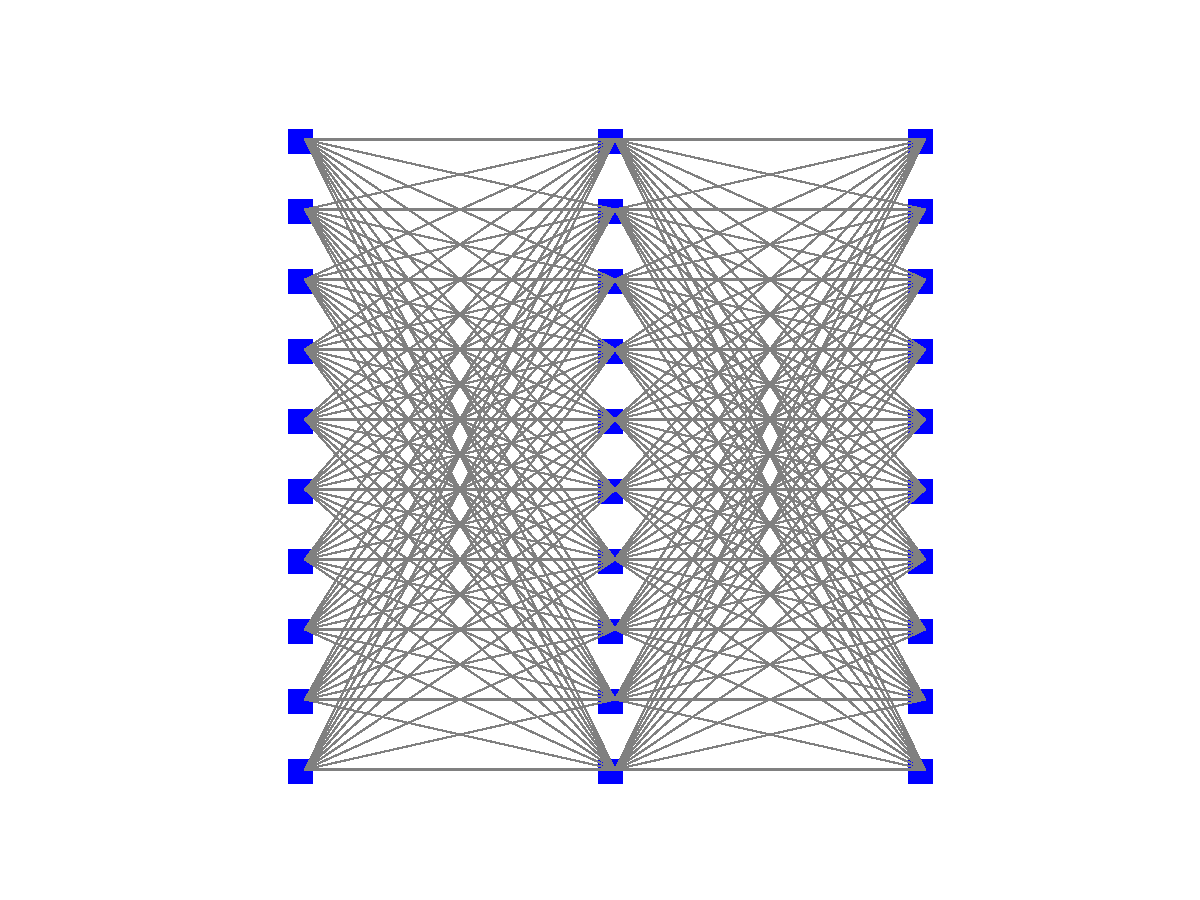
\includegraphics[width=0.8\textwidth]{Images/img9.png}
	\caption{Airbag system block diagram}
	\label{fig:Airbag system block diagram}
\end{figure}

The diagram also highlights the presence of K-line dataline protection. This component is crucial for shielding the communication lines from electrical noise and interference, ensuring that data transmission remains reliable and unaffected by external disturbances.

The wired connectivity section features CAN transceivers, which facilitate communication with other electronic control units (ECUs) within the vehicle via the CAN bus. This is essential for integrating the airbag control system with the broader vehicle electronics. To further protect this communication channel, CAN dataline protection is implemented, which prevents electrical noise from disrupting the CAN bus communication lines.

At the heart of the system is the control unit, which houses the microcontroller units (MCUs). These MCUs are built on ARM architecture, providing the primary processing power needed to handle the main control logic of the airbag system. The control unit also includes a power architecture module, which manages the distribution and power-saving modes of the system, ensuring efficient energy use. Additionally, a serial EEPROM is included for non-volatile storage of configuration data and system parameters, maintaining crucial information even when the system is powered down.

The squib drivers section is a critical part of the airbag control system. It features a System Basis Chip (SBC) that includes several key components. Voltage regulators ensure that the microcontroller and other components receive a stable power supply. The system diagnostic module continuously monitors the health and status of the system, alerting to any potential issues. Communication with diagnostic tools and external systems is facilitated by a K-line transceiver compliant with ISO9141 standards. Safety is enhanced with a dual watchdog that can reset the system in case of failure.

The SBC also includes a sensors power supply to ensure that all connected sensors receive the necessary power. Communication between the microcontroller and peripheral devices is handled via SPI buses. The SBC manages up to 12 squib drivers, which are responsible for deploying the airbags. A 4-channel satellite interface and a 9-channel DC sensor interface allow for connections with satellite sensors and DC/Hall-effect sensors, respectively. These sensors provide additional data on conditions such as acceleration, impact, proximity, speed, and position. A 3-channel general-purpose interface is also available for custom sensor connections.

An extension IC is included in the system to provide additional capacity, featuring 8 more squib drivers and another 4-channel satellite interface. This ensures the system can handle a greater number of airbags and sensors, allowing for scalability and flexibility in design.

The sensors and actuators connected to the system include squibs, which are the actuators that trigger airbag deployment, and satellite sensors that provide external data such as acceleration and impact information. DC/Hall-effect sensors detect various conditions, and warning lights indicate system status, alerting the driver to any issues.

The interface section includes PSI5 transceivers, which are used to interface with PSI5 sensors, a standard in automotive applications for reliable communication.

Data flow within the system is managed through the K-line bus, a single-wire communication line used for diagnostics and communication with external devices, and the CAN bus, a robust vehicle bus standard that allows the microcontrollers and devices to communicate without a host computer.





\subsubsection{Automotive advanced airbag IC}
In designing our advanced airbag control system, we have chosen to incorporate the L9680 IC. This chip is particularly well-suited for sophisticated airbag systems in mature markets and can also be employed in cut-off battery systems for integrated safety applications. One of the notable advantages of the L9680 is its compatibility with the L9678 and L9679 devices, allowing for seamless integration within existing safety system architectures.

The L9680 facilitates the integration of safety systems through its higher power supply currents and its built-in active wheel speed sensor interface. This interface is versatile, as it can be shared with the PSI-5 satellite interface to create a generic remote safety sensor interface that complies with both systems. This dual functionality significantly enhances the flexibility and applicability of our design.

A key feature of the L9680 is its high-frequency power supply design, which operates at 1.882 MHz. This allows for the use of smaller and more cost-effective external components, reducing overall system costs. Additionally, the integrated synchronous rectifiers within the buck converters contribute to the efficiency and reliability of the power management system.

System integrity and diagnostics are of paramount importance in our design. The L9680 addresses this by electrically isolating the ER capacitor from the boost regulator through a fixed charge current circuit, which controls in-rush current. The IC also includes a discharge current circuit to measure the capacitance and ESR of the ER capacitor, ensuring accurate diagnostics. These current sources can also be used to discharge the capacitor upon shutdown, enhancing safety.

Thanks to its low quiescent current, the L9680 can be directly connected to the battery. This enables controlled start-up and shutdown via the wake-up input function, with the power supply and crossover function managed automatically through the internal state machine.

The L9680 provides flexibility in selecting both the ECU logic voltage (either 3.3 V or 5.0 V) and the energy reserve output voltage (either 23 V or 33 V). The deployment voltage is capped at 25 V for all profiles and can be managed through an external safing switch circuit. This is controlled via the high-side safing switch reference enabled through the system SPI interface or the arming logic.


\begin{figure}[h]
	\centering
	\includegraphics[width=0.9\textwidth]{Images/img10.png}
	\caption{IC operating state diagram}
	\label{fig:IC operating state diagram}
\end{figure}















\subsection{WCET Estimation}


Based on the design and requirements provided, I will estimate the WCET for the airbag control system. Here are the steps and assumptions for the calculation:

\subsubsection{Assumptions and Details}
\begin{itemize}
	\item Sensor Access Time: Each access to a sensor or actuator takes 1 ms.
	\item Atomic Instruction Time: Each atomic instruction takes 10 nanoseconds (ns).
	\item Sensor Readings: Each sensor is read at least 3 times and at most 5 times, with the first 3 consistent readings being selected to avoid bouncing.
	\item Processor Utilization: Other tasks handled by the processor take up to 90\% of the computational power, leaving 10\% for the airbag system.
\end{itemize}

\subsubsection{Steps to Calculate WCET}
\begin{enumerate}
	\item \textbf{Reading Sensors}:
	\begin{itemize}
		\item We have four sensors \( S_1, S_2, S_3, S_4 \).
		\item Each sensor is read 3 times for consistency.
		\item Total time for reading all sensors:
		\[
		4 \, \text{sensors} \times 3 \, \text{reads/sensor} \times 1 \, \text{ms/read} = 12 \, \text{ms}
		\]
	\end{itemize}
	
	
	\item \textbf{Plausibility Check}:
	\begin{itemize}
		\item Plausibility checks involve comparing \( S_1 \) with \( S_2, S_3, \) and \( S_4 \).
		\item Let's assume this involves 3 comparisons per sensor check.
		\item Number of atomic instructions per comparison: Assume 5 atomic instructions per comparison.
		\item Total comparisons: 3 comparisons per sensor reading.
		\item Total atomic instructions:
		\[
		3 \times 3 \, \text{comparisons} = 9
		\]
		\item Time for plausibility check:
		\[
		9 \, \text{atomic instructions} \times 10 \, \text{ns/instruction} = 90 \, \text{ns} = 0.09 \, \text{µs}
		\]
	\end{itemize}
	
	
	\item \textbf{Error Handling and Decision Making}:
	\begin{itemize}
		\item If a sensor value is implausible, increment \texttt{error\_ctr}.
		\item If \texttt{error\_ctr} reaches 5, set the defect output.
		\item If plausible for 5 cycles, reset \texttt{error\_ctr}.
		\item Assume 10 atomic instructions per error handling and decision making.
		\item Time for error handling:
		\[
		10 \, \text{atomic instructions} \times 10 \, \text{ns/instruction} = 100 \, \text{ns} = 0.1 \, \text{µs}
		\]
	\end{itemize}
	
	
	\item \textbf{Firing the Airbag}:
	\begin{itemize}
		\item Determining which airbag to fire and to what extent based on the distance sensor.
		\item Assume this involves reading the distance sensor and making a decision.
		\item Sensor read: 1 ms.
		\item Decision making: Assume 10 atomic instructions.
		\item Time for decision making:
		\[
		10 \times 10 \, \text{ns} = 100 \, \text{ns} = 0.1 \, \text{µs}
		\]
		\item Total time for firing decision:
		\[
		1 \, \text{ms} + 0.1 \, \text{µs} = 1.0001 \, \text{ms}
		\]
	\end{itemize}
	
	
	
	\item \textbf{Additional Considerations}:
	\begin{itemize}
		\item Total cycles for plausibility: 5 cycles.
		\item Total time for plausibility cycles:
		\[
		5 \times (12 \, \text{ms} + 0.09 \, \text{µs} + 0.1 \, \text{µs}) = 5 \times 12.0002 \, \text{ms} = 60.001 \, \text{ms}
		\]
	\end{itemize}
\end{enumerate}



\subsubsection{Total WCET Calculation}
\begin{align*}
	\text{Total WCET} &= \text{Sensor readings} + \text{Plausibility checks} + \text{Error handling} + \text{Firing decision} \\
	&= 60.001 \, \text{ms} + 1.0001 \, \text{ms} \\
	&= 61.0011 \, \text{ms}
\end{align*}

\subsubsection{Adjusting for Processor Utilization}
Only 10\% of the processor's computational power is available for the airbag system. Therefore, the effective time available for the airbag system is:
\[
10\% \times 61.0011 \, \text{ms} = 6.10011 \, \text{ms}
\]

\subsubsection{Final WCET}
The final WCET, considering the processor utilization, is approximately \textbf{6.1 ms}.














\subsection{Real-time Checking}
Ensuring that the airbag control system operates in real-time is critical for the safety and reliability of the vehicle. Based on the WCET (Worst-Case Execution Time) calculations and the design considerations, \textbf{I can confidently state that the timing constraints will be met}, ensuring the system operates within the required real-time parameters. By integrating the STM32 microcontroller with the L9680 IC and implementing an interrupt-based design, I can guarantee that the airbag control system meets the stringent real-time requirements necessary for safe and reliable operation. The calculated WCET of 6.1 milliseconds, combined with robust safety mechanisms, ensures that the system can respond promptly and accurately to collision events, providing optimal protection for vehicle occupants. Thus, the design confidently meets and exceeds the necessary real-time performance standards.

The STM32 microcontroller's advanced features, combined with the L9680 IC, offer an ideal platform for implementing a high-performance airbag control system. The WCET of 6.1 milliseconds ensures that the system can process sensor data, perform plausibility checks, and make deployment decisions well within the critical timeframes required for effective airbag deployment. The L9680 IC's high-frequency power supply design, operating at 1.882 MHz, allows for the use of smaller, less expensive external components, reducing system costs while maintaining high performance. The integrated synchronous rectifiers in the buck converters enhance efficiency and reliability, ensuring stable power delivery to the system.

An interrupt-based design on the STM32 microcontroller ensures immediate response to critical events. The NVIC (Nested Vector Interrupt Controller) allows for efficient management of multiple interrupts, ensuring that high-priority tasks, such as airbag deployment, are processed without delay. This design minimizes latency and maximizes the responsiveness of the system. The L9680 IC includes multiple safety features, such as the isolation of the ER capacitor from the boost regulator and integrated discharge current circuits for measuring capacitance and ESR. These features ensure system integrity and prevent accidental deployments, enhancing overall safety.

The airbag control system performs rigorous plausibility checks on sensor data to prevent false positives. Sensor values are cross-checked for consistency, and if values are implausible, the system increments an error counter. If the counter reaches a threshold, the system sets a defect output and shuts down, indicating a sensor fault and preventing erroneous airbag deployment. This robust error handling mechanism ensures that the airbag system only activates in genuine collision scenarios. The L9680 IC allows for flexibility in selecting ECU logic voltage (3.3 V or 5.0 V) and energy reserve output voltage (23 V or 33 V), with deployment voltage capped at 25 V for all profiles. This flexibility, combined with the STM32 microcontroller's scalability, allows the system to be tailored to specific vehicle requirements and future expansions.

Continuous real-time monitoring of system health and status through the L9680 IC's diagnostics capabilities ensures that any issues are promptly detected and addressed. This proactive monitoring enhances the reliability and safety of the airbag control system. In conclusion, the integration of the STM32 microcontroller with the L9680 IC, coupled with an interrupt-based design, ensures that the airbag control system meets the stringent real-time requirements essential for safe and reliable operation. The calculated WCET of 6.1 milliseconds, along with comprehensive safety mechanisms and robust error handling, guarantees that the system can respond swiftly and accurately to collision events, providing optimal protection for vehicle occupants. This design confidently meets and exceeds the necessary real-time performance standards, ensuring the highest levels of safety and reliability.






\newpage

\section{Elevator System}


\subsection{Project Description}
You have probably had a frustrating experience using the elevator in the east wing of the faculty. The goal in designing this elevator was that by pressing a button again (either on the floors or in the cabin), the command to move to that floor would be canceled. However, the timing of this second press (whether before starting to move towards that floor or during the movement) was not properly considered. Additionally, the designer intended that if the elevator could not move, the call request would be canceled (timeout). Unfortunately, this part of the system does not function correctly in practice either.



\subsection{Project Detail}
In this part of the project, provide a complete description of the correct behavior of the faculty's elevator using a Petri net. In other words, suppose that while retaining the features of the existing elevator, you want to provide an accurate description to fix its current issues. You can base your description on a simple elevator system using a Petri net that you have seen in the course. However, keep in mind that the number of floors in this problem is known (4 floors in the faculty), and the current features of the elevator (including cancellation by pressing again and timeout) must remain. For simplicity, there is no need to perform a qualitative analysis and evaluation of the description. However, if you do perform this analysis and evaluation, you will receive additional points.

Note: \textcolor{red}{This provides a good opportunity for students who did not manage to earn good marks in other parts of the course to make up for this weakness through the project's bonus sections.}












\newpage
% ----------------------------------------------------------------------
% References
% ----------------------------------------------------------------------
\bibliographystyle{plain}
\bibliography{refs}

\end{document}